\chapter{Problemanalyse}\label{ch:analyse}
I dette kapitel undersøges den initierende problemstilling. Der redegøres for, at det faktisk er et problem, og ikke bare noget gruppen har antaget er et problem. Således ender projektet med at løse noget aktuelt. Yderligere redegøres der for, hvem dette er et problem for. Kapitlet ender ud i en afgrænset problemformulering, som skal lede projektet fra problemet til en løsning.

\section{Administration og IT i virksomheder}
I dette afsnit vil der lægges fokus på hvilke konsekvenser it administration har for små virksomheder. Dette inkluderer fordele og ulemper ved IT systemer samt virksomhedernes nødvendighed i at holde sig konkurrencedygtige. Afsnittet underbygger den initierende problemstilling og undersøger de eksisterende positive og negative sider af IT administration. Dette opnås ved at undersøge en række kilder for relevant data om IT administrations effekt på arbejdsmiljøet og konkurrencedygtigheden.\\

Det bliver vigtigere for virksomheder at benytte IT redskaber til administrativt arbejde og til at få virksomhedens daglige rutine til at fungere. Uden IT falder virksomheder konkurrencemæssigt bagud, da de ikke er i stand til at udføre opgaver lige så effektivt som deres konkurrenter. Væsentligheden af IT beskrives således af information og rådgivnings firmaet IBiz Center: \textit{"IT-integration er alfa og omega"} \citep{case_green_team}. Desuden kan IT systemer bruges til at løse en række forskellige administrative opgaver på en gang. Færre processer gør, at det bliver nemmere for ledelsen at udføre dem \citep{Ibiz_streamline}. Ved brug af IT systemer, i stedet for manuelle- eller papirsystemer, kan integriteten af tal og informationen desuden sikres. Således sikres personalet ikke at få for lidt i løn, kunder får de rigtige varer og tjenester og varer ligger på de angivne placeringer i lageret osv. \citep{Ibiz_streamline} Ved at benytte et system, der undersøger om dataen er korrekt, kan virksomheden både spare tid og penge \citep{case_green_team}. 

\newpage
\subsection{Cloud computing}
Uanset hvilken sektor og branche en virksomhed befinder sig i, sker der en stigning i brug af IT som set på figur [\ref{fig:virksomcc}]. Figuren viser stigningen af \textit{"Virksomheder der anvender cloud computing"} fra år 2012 til 2014. Selvom cloud computing ikke er den eneste form for IT løsning til virksomheder, står den for over en tredjedel af de anvendte IT løsninger, og er derfor ikke ubetydelig. Der kan uddrages vigtig information om IT-brug fra Dansk Statistiks data om cloud computing \citep{itvirk}. Den data der uddrages er, hvilke typer af virksommheder, som bruger cloud computing. Desuden kan det ses hvor stor en procentdel anvendelsen stiger pr. år. Den mindste stigning fra 2012 til 2014 er på 11\%, imens den største er på 25\%. Hvis andre indenfor en sektor bruger IT, så bliver det vigtigt for, specielt nye og mindre, virksomheder  at bruge det, for at kunne følge med i udviklingen.  
\newpage
\begin{figure}[H]
    \centering
    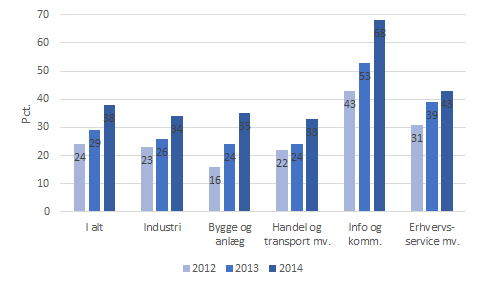
\includegraphics[width=1\textwidth]{figures/CloudComputingStatestik.png}
    \caption{Statistik over virksomheder, som benytter cloud computing \citep{itvirk}} 
    \label{fig:virksomcc}
\end{figure}

\begin{figure}[H]
    \centering
    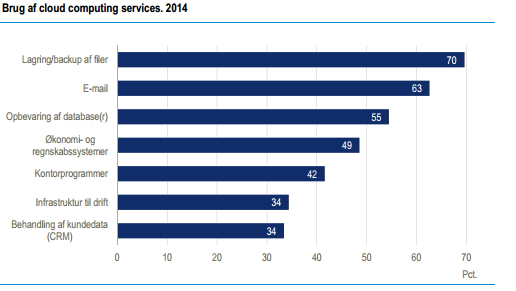
\includegraphics[width=1\textwidth]{figures/brugafccservices.png}
    \caption{Statistik over distribution af Cloud Computing brug \citep{itvirk}}
    \label{fig:distcc}
\end{figure}

\newpage
På figur [\ref{fig:distcc}] ses det, at over halvdelen af virksomhederne, som anvender cloud computing, bruger løsningen til opgaver som filhåndtering og database brug, samt e-mail. Disse ting udgør ca. 63\% af al cloud computing brug i virksomheder. Yderligere vises det at over en tredjedel benytter det til infrastruktur, kundedata, økonomi mm. Cloud computing mindsker også mængden af tid der bruges på vedligeholdelse af systemet da udbyderen af cloudcomputing er ansvarlig for vedligeholdelsen. 

Dog skal det bemærkes at cloud computing ikke er en perfekt løsning. et eksempel er cloud storage servicen Dropbox. På deres hjemmeside står der, at de stræber efter \textit{"100\% uptime"} men at \textit{"det er urealistisk at garentere det"} \citep{drpbx_downtime}. Ved brug af cloud computing er det vigtigt at være opmærksom på den downtime servicen el.lign. har. Nogle services kan f.eks. have downtime i løbet af ugen, hvis de skal vedligeholde deres udstyr.

\subsection{Hvorfor cloud computing?}
Systemer lavet til virksomhedsbrug kaldes for enterprise computing. Software, der benyttes til administration af virksomheder, falder ind under denne kategori. Som McKendrick's artikel forklarer det, er enterprise  computing "on-approval, static, private, purchased, and fundamentally inaccessible" \citep{McKendrick2014}. Hvilket er det modsatte af hvad der forstås ved cloud computing, som er elastisk, on-demand og tilgængelig \citep{McKendrick2014}. I bogen \textit{Enterprise cloud computing : technology, architecture, applications} undersøger og beskriver Shroff internettets udvikling, til at blive en cloud computing platform \citep{Shroff2010}. Grundet naturen af hvordan cloud computing virker, er det muligt for brugeren af en sådan service, kun at betale for den benyttede data \citep{Shroff2010}. På den måde skal hverken serviceudbyderen eller brugeren stå med en masse plads (i tilfældet af cloud storage) eller lignende, som ikke kan benyttes. %For dette projekt betyder det, at hvis der er tid til at udvikle en cloud baseret løsning,


\subsection{Konsekvenser for arbejdsmiljøet}
Cloud computing har det aspekt, at det er allestedsnærværende. Uanset hvor en medarbejder befinder sig, enten på arbejde eller derhjemme, er der mulighed for at arbejde. I toget, derhjemme eller til møde er det er altid muligt at tilgå sine dokumenter, e-mails, applikationer, osv. Flere virksomheder benytter dette, så deres medarbejdere kan bruge mere energi på deres arbejde. Når en ansat altid har arbejdet med sig i form af pc, tablets, smartphones, osv. gør dette at arbejdet altid kan tilgås. Der er altså tale om \textit{"det grænseløse arbejde"} \citep{SystimeStress}, da der nu er mulighed for at tage arbejdet med hjem. Det grænseløse arbejde, er blevet mere udbredt i forbindelse med samfundets udvikling, da der sker en stigning af folk med karrierelivsformen samt, at teknologien gør det lettere at have denne livsform. At være fleksibel er derfor blevet en præmis indenfor arbejdsmarkedet. Denne udvikling giver det fleksible menneske flere muligheder i form af job og uddannelse, men medfølger at arbejdslivet er blevet mere uforudsigeligt. Fleksibilitet kan derfor have en stressende effekt, og det er derfor vigtigt at tage hensyn til dette i implementationen af en løsning. Dette kan være svært ud fra et datalogisk synspunkt, da stress ikke er noget der kan måles eller vejes. \citep{SystimeStress}

\subsubsection{Opsummering}
IT administration er en essentiel del for virksomheder der vil være konkurrencedygtige. Cloud computing står for over en tredjedel af it løsninger som virksomheder bruger - et brug som stiger hvert år. Cloud computing bliver brugt til en lang række opgaver, hvor ca. 63\% af virksomhederne bruger det til e-mail, filhåndtering og database brug. Over en tredjedel benytter det til infrastruktur, kundedata og økonomi. Cloud computing er dog også allestedsnærværende, hvilket vil sige, at arbejdet kan tages med overalt. Dette kan have en stressende effekt, hvilket vil påvirke arbejdsmiljøet.




%Når nye IT systemer bliver implementeret er det vigtigt at der er styr på at de fungerer korrekt. Der er tilfælde hvor nye IT systemer ikke har fungeret optimalt. Dette kan observeres ved systemer som fx ”amanda” eller ”EFI” som kostede staten over 1 milliard kroner, uden at blive sat i brug \citep{DrItsys}. \todo{Syntes det virker lidt hurtigt skrevet og meget kort -- Er det her faktisk relevnt for denne section? og i så fald så skal systemerne uddybes i stedet for bare at nævnes. Smed} I takt med at mindre virksomheder udvider, samt den konkurrence imellem virksomheder, er der stigende krav til kvantitaviteten og tempoet hos administrationen i virksomhederne. Denne ekstra belastning kan resultere i dårlige arbejdsforhold, hvilket vil sænke produktiviteten yderligere. Et IT-værktøj til at afhjælpe i administrations delen ville kunne lette en sådan belastning og dermed forbedre arbejdsmiljøet \citep{It_armil}. 



\section{Arbejdsmiljø} \label{arbejdsmiljoe}
Dette afsnit analyserer IT administrations indvirkning på arbejdsmiljøet samt hvilke konsekvenser et dårligt arbejdsmiljø har på en arbejdsplads og medarbejderne. Afsnittet tager udgangspunkt i kilder til stress på arbejdspladser og eksempler på arbejdspladser som anvender IT administration. Afsnittet undersøger om mangel på IT administration kan have en negativ påvirkning på en arbejdsplads, og om det skaber et ineffektivt arbejdsmiljø \citep{Cambridge2011}.\\

Videncenter for arbejdsmiljø har lavet en definition på begrebet arbejdsmiljø som lyder således: \textit{"Arbejdsmiljø er et samspil af de relationer, påvirkninger og vilkår, som mennesket arbejder under. Det er også den tekniske og sociale udvikling af arbejdspladsen, som kan bidrage til det enkelte menneskes sikkerhed på kort sigt samt til menneskets fysiske og psykiske sundhed på længere sigt"} \citep{Arbejdsmiljoe}. Det kommende afsnit omhandler forskellige indvirkninger på arbejdsmiljø. Det forklares hvordan IT administration kan have en indvirkning på arbejdsmiljøet. Et arbejdsmiljø kan have mange forskellige påvirkninger på medarbejderen. Dette inkluderer:

\begin{itemize}
    \item {\textbf{Psykisk påvirkning} \citep{Arbejdsmiljoe_psykisk}}
    \begin{itemize}
    \item {\textbf{Stress}: At arbejde kan være stressende, og dette kan have indvirkning på både arbejderen og arbejdsmiljøet. Stress kan f.eks. give hukommelsesbesvær, koncentrationsbesvær og nedsat humør. Disse faktorer kan både påvirke arbejderens arbejdsproces og arbejderens arbejdsomgivelser. \citep{Arbejdsmiljoe_stress}}\\
    \end{itemize}
    \item {\textbf{Fysisk påvirkning} \citep{Arbejdsmiljoe_fysisk}}
    \begin{itemize}
    \item {\textbf{Slid}: Et arbejde kan være fysiskt hårdt på mange måder. Dårlige muse anordninger til computerbrug kan f.eks. resultere i skader i håndled. \citep{Arbejdsmiljoe_fysisk}}
    \item {\textbf{Støj}: En larmende arbejdsplads kan også have stor indvirkning på arbejderens hørelse, i form af fysiske høreskader og er også en faktor til psykisk stress. \citep{Arbejdsmiljoe_stoej}}
    \item {\textbf{Klima}: Aspekter som for høj eller for lav temperatur (højere end 25 grader, lavere end 20 grader), og et indelukket eller forurenet klima, kan have fysisk påvirkning på medarbejderen i form af f.eks. tørre øjne, træthed og hovedpine. \citep{Arbejdsmiljoe_indeklima}.}\\
    \end{itemize}
\end{itemize}

Med henblik på IT administration, kan den negative påvirkning forekomme, når der er en mangel på effektiv IT administration, som f.eks. over-krævende- og ufleksible arbejdsplaner, hvilket kan resultere i stress hos den enkelte medarbejder \citep{Cambridge2011}.

\subsection{Vagtplanens indflydelse på arbejdsmiljø}
For at forebygge konsekvenserne af et dårligt arbejdsmiljø, er en struktureret eller fleksibel vagtplan en mulighed. En fleksibel vagtplan, hvor medarbejderen er med til at vælge sine vagter, vil udover at skabe et bedre arbejdsmiljø også ansvarliggøre den enkelte medarbejder. En fleksibel vagtplan vil sikre et bedre arbejdsmiljø, ved at skabe større fleksibilitet mellem arbejde og privatliv. Det øgede ansvar giver også medarbejderen en forståelse for arbejdsplanlægningen og skaber dermed et større engagement i at få arbejdsplanen til at gå op. Samtidig vil vagtplanlæggeren få mere tid til andet arbejde som f.eks. kvalitetssikring.
Undersøgelser viser også, at gode og fleksible arbejdstider er fastholdelses potentiale for medarbejderne, hvilket vil sige at kontinuiteten opretholdes. \citep{It_armil} 

\subsection{Fleksibel arbejdstid}
Dette afsnit tager udgangspunkt i artiklen: \textit{Ny fleksibel arbejdstid gav mere arbejdsglæde} \citep{Thomse2014}. På et plejehjem blev der implementeret et IT-system, hvor medarbejderne selv skulle vælge deres vagter. Ifølge artiklen blev IT-systemet indført fordi \textit{"at man gerne vil forebygge overbelastning af de stadig færre, der vælger at arbejde i sektoren og dermed også både fastholde dem i jobbet og rekruttere nye."} IT-systemet har givet medarbejderne mere frihed, da muligheden for selv at vælge vagter, gør det lettere at tilpasse sig. Systemet virker ved at medarbejderne starter i en ønske fase, hvor de vælger de tider og dage de helst vil arbejde. Herefter bliver ønskerne puslet sammen i fællesskab, sådan at der altid er et tilstrækkeligt antal medarbejdere på arbejdet. Plejehjemmet udmelder at i denne sammenhæng, kan det være fornuftigt at have en blanding af medarbejdere der har, og ikke har børn. Denne fleksible IT løsning reducerer også de mistænkelige sygedage (dage hvor folks sygedom betvivles), fordi at medarbejderne selv fik mulighed for at vælge, hvilke dage de ville have fri. Den generelle stemning på arbejdspladsen er også blevet væsentligt bedre, da medarbejderne selv har valgt deres vagter, hvilket gør det svært at være utilfreds med arbejdstiderne. IT-systemet har derimod ikke kun været godt. I starten forholde nogle af medarbejderne sig konservativt til løsningen og var tilfredse med vagtsystemet som de havde før. Efterhånden begyndte næsten alle dog at kunne se fordelene ved det nye IT-system. 
\\Der kan altså uddrages at på en arbejdsplads som et plejehjem, hvor der skal være folk på arbejde hele tiden, at det er en fordel for medarbejderene at have indflydelse på hvilke tidspunkter de gerne vil arbejde, da det kan være en smule anderledes i forhold til en arbejdsplads uden bemanding døgnet rundt, med faste arbejdstider. Derfor kan det være en fordel, hvis der er forskellige typer af mennesker. Folk med børn kan have det bedre med normale tider, altså der passer sammen med deres børns skole, fritid, osv. hvor at en medarbejder uden børn har lettere ved at tage de lidt mere atypiske vagter. Der er altså tale om en kategorisering af medarbejdere. Muligheden for valg af vagter og opgaver der følger med disse, kunne også have forbindelse med de færre mistænkelige sygedage, da medarbejderen får mere ansvar, hvilket kan give et bedre arbejdsmiljø \citep{Sygdag}.

\subsubsection{Opsummering}

IT administration har en indvirkning på et givet arbejdsmiljø. Dette sker dog på det psykiske plan. Stress er et eksempel på en psykisk påvirkning som resultat af ineffektiv IT administration. På den anden side så skaber en god IT administration et godt arbejdsmiljø. Udover det faktum at en arbejdsplads medarbejdere er gladere i et godt godt arbejdsmiljø, så resulterer et godt arbejdsmiljø også i en mere effektiv arbejdsplads.

\section{Interessentanalyse}
I dette afsnit undersøges de parter som har interesse i arbejdsplanlægning. Dette gøres gennem analyse af interessentens fokusområder på problemet samt hvilke krav de har til en eventuel løsning af problemet.

Med henblik på et givet problem, vil der være interessenter, der bliver påvirket. Herved bliver interessentanalysen brugt til at finde de interessenter, der er interesserede i at løse problemer angående ineffektiv administration og IT i små virksomheder, med henblik på planlægning.
Derfor er denne analysemodel nyttig til at identificere de vigtigste interessenter, sådan at der kan tages forbehold for interessenternes ønsker og behov i en eventuel løsning af problemet. Efter at interessenterne er identificeret gennem brainstorming, bliver de placeret i en Indflydelse og Medvirken Matrix \ref{fig:PavirkInflydMat}, som opdeler interessenterne i fire kategorier. Herefter bliver interessenterne opdelt i prioriteret rækkefølge med henblik på vigtighed for problemløsningen.

\begin{figure}[H]
\centering
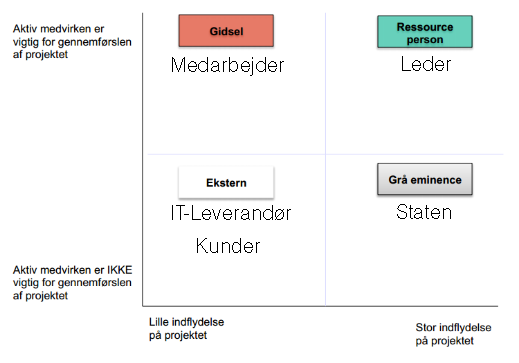
\includegraphics{figures/IndflydelsePaaMatrixMedInteress.png}
\caption{De vigtigste interessenter placeres i Indflydelses og påvirkningsmatrixen}
\label{fig:InteressentMatrix}
\end{figure}

\subsection{Medarbejder}
Medarbejdere er påvirket af problem, da de, i kraft af deres arbejde, kan blive udsat for dårlig arbejdsplanlægning, som bidrager til et dårligt arbejdsmiljø. Deres samarbejde er vigtig for løsning af problemet, da implementeringen afhænger af medarbejdernes samarbejdsvillighed. Selvom deres deltagelse er vigtig, har de ikke nogen indflydelse på løsningens udformning. Det vil oftest være en leder, som står for arbejdsplanlægningen og dermed anvender de blot den gennemarbejdede arbejdsplan. Medarbejdernes holdninger til projektet kan variere alt efter hvilken erfaring de har med det nuværende system. Det kan f.eks. være problematisk at skulle sættes ind i et nyt system, hvis de lige har lært at bruge det nuværende. Dog kan det også være at løsningen tilvejebringer en bedre måde for dem at håndtere deres arbejdsplan, hvorved de får mere overblik over deres arbejdstider. Medarbejderne er sat ind i figur \ref{fig:InteressentMatrix} som gidsler. De er placeret her fordi at de hovedsageligt bliver påvirket af problemet, da det er dem der anvender arbejdsplanlægningen, men ikke har nogen indflydelse på løsningen af problemet.

\subsection{Leder}
Lederen er interesseret i problemet, da det primært er dem som holder overblik over medarbejderne. Derfor er lederen vigtig for forståelsen af problemet, da det er dem som har erfaring indenfor planlægning og kender de nuværende behov til arbejdsplanlægning. Ifølge artiklen "4 trin til planlægning der holder", er lederen interesseret i effektive planlægnings værktøjer fordi, at disse giver lederen et større overblik og bedre fokus, hvilket gør virksomheden mere effektiv \citep{Kolding2012}. Lederen er en ressourceperson \ref{fig:InteressentMatrix}, fordi at lederen både har en påvirkning på problemløsningen,  og fordi lederens medvirken er vigtig for løsningen.

\subsection{IT-leverandør}
IT-leverandøren er det firma som sælger og udvikler IT-softwaren. De leverer systemer, som hjælper virksomheden med administration. IT-leverandøren, bliver ikke påvirket af problemet, men er interesseret i at (hjælpe med at) løse det. De sørger for at softwaren, bliver installeret og gjort køreklar for virksomheden, efter softwaren er udviklet. Derfor er IT-leverandøren sat som en Ekstern interessent, som kan ses i Figur \ref{fig:InteressentMatrix}.

\subsection{Kunde}
Kunderne for firmaet er en interessent, da de modtager den service som firmaet tilbyder og er derfor direkte påvirket af firmaets effektivitet. Kunderne er brugere af firmaet, men de har ikke nogen indflydelse eller medvirken på problemløsningen. De bliver indirekte påvirket af problemet, hvilket er grunden til at de ikke har nogen indflydelse på udformningen af løsningen. Kunderne er derfor sat som Ekstern \ref{fig:PavirkInflydMat}.

\subsection{Staten}
Staten har en interesse i at sikre et godt arbejdsmiljø i Danmark. De er interesserede i at mindske stress på arbejdsmarkedet. Et eksempel på dette er deres kampagne \textit{"Fra stress til trivsel"}\citep{Arbejdsmiljoe_Arbejdspladser}. Statens kampanger tilbyder arbejdspladserne materiale og ressourcer til løsning af eventuelle stress relaterede problemer, men arbejdspladsen skal selv stå for at udnytte ressourcerne. Staten er derved ikke interesseret i selv at skulle bestemme på hver eneste arbejdsplads. Derfor har de ikke stor indflydelse eller medvirken i løsningen af problemet. Beskæftigelsesministeriet er en del af staten og det er deres opgave at fremlægge lovforslag til arbejdsmiljøloven, samt sikre at lovene bliver opretholdt \citep{Beskaeftigelsesministeriet2002}.

\subsubsection{Arbejdstilsynet}
Arbejdstilsynet er en del af Beskæftigelsesministeriet og har til opgave at sikre et bedre arbejdsmiljø i Danmark. Arbejdstilsynets opgave er, at sikre  arbejdsforholdene på de danske virksomheder er sikkerheds- og sundhedsmæssigt fuldt forsvarlige, på baggrund af arbejdsmiljøloven \citep{Arbejdstilsynet2015}. Virksomhederne er derfor nød til at lave deres vagtplaner med baggrund i lovene om arbejds- og hviletider. På den måde står staten og arbejdstilsynet som en grå eminence \ref{fig:PavirkInflydMat}, da de fastsætter og håndhæver en række love, som har indflydelse på problemet, men som samtidig ikke har stor medvirken i løsningen af problemet \citep{Beskaeftigelsesministeriet2002}.

\subsection{Prioriteringen af interessenter}
Ud af de seks førnævnte interessenter, er de vigtigste udvalgt med henblik på en problemløsning, i forhold til arbejdsmiljø. Disse interessenter bliver sat i prioriteret rækkefølge, som henholdsvis primære, sekundære og tertiære interessenter. Lederne blev udvalgt som den primære interessent, da de styrer virksomheden og står for arbejdsplanlægningen. Dermed er det også dem, der sidder med problemet, at ligge en arbejdsplan, og vil derfor også få mest ud af en eventuel løsning. Hvis arbejdsplanlægningen ikke foregår optimalt, kan det få konsekvenser for hele virksomhedens arbejdsmiljø. Medarbejderen blev udvalgt som sekundær interessent, da de bliver påvirket af problemet men ikke bestemmer hvilken vagtplanlægnings løsning, der bliver anvendt. De bliver påvirket af en en dårlig vagtplan, hvilket kan skabe et dårligt arbejdsmiljø. Staten blev udvalgt, som en tertiær interessent, da staten har til opgave at skabe retningslinjer indenfor arbejdsmiljø og arbejdstider.

\subsubsection{Opsummering}
I interessentanalysen blev de de grupper der kunne være interesseret i en vagtplanlægningsløsning fundet. Udover blev de også kategoriseret efter hvor højt de skulle prioriteres. Det blev gjort efter hvor meget indflydelse og medvirken de havde i en given arbejdsplanlægningssoftware. Dem der havde stor inflydelse og medvirken blev prioriteret højst, og dem der havde lav medvirken og indflydelse blev prioriteret lavere. Efter kategoriseringen så blev de sat ind i en Påvirkning og Indflydelses Matrix.

\section{Interview}
Dette afsnit bliver brugt til at bygge videre på interessentanalysen, for at finde ud af hvad interessenterne vil have i en given løsning. Derudover bruges interviewsene til at finde ud af hvad for nogle eksisterende løsninger virksomhederne bruger, som vi så kan analysere på senere i rapporten. 

Ved hjælp af interessentanalysen, er det blevet klargjort, hvilke personer der er interesserede i problemet. Ved interviewene stræbes der efter at opnå en viden omkring hvilke problemer der er ved nuværende løsninger, samt krav til fremtidige løsninger. Interviewsene blev herefter brugt til at skabe indsigt indenfor emnet. Spørgsmålene blev lavet på baggrund af nogle emner der skulle belyses. Udfra disse emner, blev nogle korte og åbne spørgsmål lavet, for at sikre, at den viden der opstod blev reflekteret over. Dette ville ikke være muligt med f.eks. ledende spørgsmål, hvor interviewpersonen bliver påvirket i en bestemt retning. Ved hjælp af svarene fra interviewsene blev det gjort klart, hvilke problemer der var med de nuværende systemer, samt positive sider heraf. %Udfra disse data kunne en foreløbig kravspecifikation dannes.

Det kvalitative forskningsinterview forsøger at forstå verden fra interviewpersonens synspunkt, herunder meninger og holdninger \citep{kvale2009}. Viden i forskningsinterviewet skabes i interaktionen mellem interviewer og interviewperson \citep{kvale2009}. Interview er valgt frem for et spørgeskema, da den viden intervieweren opnår ved et interview, ikke nødvendigvis ville opstå i en spørgeskemaundersøgelse. Interview giver interviewpersonen mulighed for at fordybe sig i og udforske egne oplevelser og meninger \citep{kvale2009}. Den viden der opnås ved et interview, er socialt konstrueret, da det ikke bare er en dataindsamling, men at der skabes data gennem den førnævnte interaktion \citep{kvale2009}.

\subsection{Analyse af interviews}
De seks interviews blev foretaget i seks forskellige butikker for at sikre diversitet blandt interviewpersonernes svar. Dette sikrede også indsigt i hvilke vagtplanlægningssystemet forskellige virksomheder anvender, samt de fordele og ulemper som interviewpersonerne har oplevet ved systemet. 

\subsubsection{Home}
Home er en ejendomsmægler kæde med 159 butikker. Den interviewede butik har 3 fultidsansatte. Denne butik er blevet interviewet for at skabe diversitet blandt interviewbutikkerne og for at undersøge arbejdsplanlægningen i en mindre butik. I interviewet med Home blev det klart at afdelingen ikke benytter sig af  et specialiseret vagtplanlægningssystem. I stedet anvender de en fast kalender. Dette er blandt andet fordi afdelingen har tre ansatte og det er derfor ikke nødvendigt at have mange på arbejde, samt at de ansatte var fuldtidsansatte. Dette giver ikke et behov for en fleksibel arbejdsplan, men i stedet en struktureret plan der er fastlagt for en længere periode. Vagtplanen blev lagt med tre ugers mellemrum, hvilket giver fleksibilitet på langtsigt. Processen med at lave en vagtplan bliver beskrevet således: \textit{”Der bliver lavet i en manuel kalender først, så bliver det bare proppet ind i kalenderen deroppe”} [\ref{app:home}]. Dette tydede på, at det er en simpel proces. Dette hænger sammen med, at de ikke var mange i afdelingen samt at de var fuldtidsansatte. Fuldtidsansatte arbejder 37 timer i ugen, og dermed er der ikke et stort behov, for at ændre på vagtplanen, da ingen har sammenhængende fridage. Vagtplanen bliver udarbejdet manuelt og derefter synkroniseret med medarbejdernes Outlook konti. Systemet har den fordel at medarbejderne ikke skal sættest ind i brugen af et nyt system. Det kan være en ulempe hvis antallet af medarbejdere bliver større da chefen selv skal tilrettelægge vagtplanen. [\ref{app:home}]

\subsubsection{Friluftsland}
Friluftsland er en enkeltstående specialbutik i Aalborg. Butikken har ?? ansatte som bemander butikken i timerne fra 10.00 til 17.30 i hverdagene. Butikens ansatte er deltidsansatte og har derfor skiftende arbejdstider igennem hele ugen. Friluftsland benytter vagtplanlægningssystemet Staffweb. Programmet anvendes af butikschefen til at udarbejde en vagtplan for en længere periode. Derefter kan medarbejderne tilgå vagtplanen via programmet på deres computere. Staffweb tilbyder dog også flere funktionaliteter en arbejdsplanlægning. Butikschefen fortæller at programmet lægger stor vægt på, at der skabes et overblik over butikken og medarbejdere i Staffweb. Her er taxerne for de forskellige dage samt de forskellige medarbejdere lagt ind, sådan at der hele tiden kan ses et samlet overblik over lønbudgettet. Derudover, opstiller programmet statistikker over hvor ofte medarbejderne bytter deres vagter og tager ledige vagter. Ved bytning af vagter, bliver vagterne lagt op i en bytte-børs som alle medarbejderne kan tilgå. Dog skal medarbejder kontakte butikschefen for at få vagtbytningen godkendt. Der bliver også skabt overblik over, om medarbejderne møder ind til tiden, da de skal stemple ind når de møder. Igen giver dette et overblik over hvilke medarbejdere der møder til tiden og hvilke der ikke gør. [\ref{app:friluftsland}]

\subsubsection{Kiwi}
Kiwi er en dagligvarekæde med 108 butikker i Danmark. ?? ansatte I butikken hvor dette interview blev foretaget er åbningstiderne mellem 7.00 til 23.00 i hverdagene og 8.00 til 21.00 i weekenderne. %http://kiwi.dk/wp-content/uploads/2015/01/KIWI-fjerner-momsen-p%C3%A5-%C3%B8kologisk-k%C3%B8d.pdf
I interviewet med Kiwi blev det klart at Kiwi benytter sig af samme vagtplanlægningssystem som Friluftsland [\ref{app:kiwi}]. Som det bliver beskrevet i interviewet med Kiwi, fungerer Staffweb systemet bedre end det tidligere papirformssystem som de anvendte;\textit{ “I forhold til før hvor vi havde det på papiret, der er det nemmere, fordi enhver har ikke undskyldningen med, min vagtplan er blevet væk, fordi man kan altid bare gå ind på nettet, også trykke, og for det er en simpel kode og et simpelt brugernavn som er bestemt af firmaet, så man kan altid finde det, så det er en klar fordel i forhold papir vagtplaner, bare det at det ikke kan blive væk, man har aldrig undskyldning, det vidste jeg ikke”}. Butikskæden ansatte er primært deltidsansatte og ungearbejderne hvilket skaber et behov for en fleksibel vagtplan, og ud fra ovenstående citat, kan det uddrages, at Staffweb systemet hjælper medarbejderne med at bevare en fleksibilitet i deres vagtplan. Da dagligvarer butikker ofte har mange deltidsansatte, gør dette også, at vagtbytning, mellem de ansatte, oftere hænder. Dette sker ligeledes ved, at chefen bliver kontaktet, sådan at vedkommende er informeret om, at en vagt er blevet byttet;\textit{ “Vi vil have det på sms, sådan så at vi kan sige, du skrev til mig og det er sådan det er, så kan vi altid have det”}. Dette gøres som dokumentation sådan at butikschefen altid er sikker på at de ansatte måder til deres vagter.
I interviewet blev en mangel ved Staffweb systemet beskrevet således: \textit{“Systemet mangler den ting, at når en medarbejder stopper, at man så kan fortsætte vagtplanen i en anden persons navn, du kan ikke bare rykke, sige alle den persons vagter, skal flyttes over til den person”}. Dette tyder på at der er et behov for at kunne nemt overfører en vagter fra en person til en anden. [\ref{app:kiwi}]

\subsubsection{Netto}
Netto er en dagligvarerbutik med 459 butikker i Danmark. Butikken ansetter oftest deltidsansatte og ungearbejdere. Butikken har åbent mellem 7.00 og 21.00 mandag til lørdag. I Netto anvendes systemet Timeplan. Systemet er designet med henblik på at give lederen overblik over økonomi, hvilket gør at lederen igen ikke skal bruge mange ressourcer på at opgøre medarbejdernes løn:\textit{ “Det regner lønnen ud også. Hvor meget man lægger til at bruge om måneden på året og på ugen og på dagen, alt. Og selv for at man får helligdagstillæg aftentillæg jeg skal ikke ligge noget som helst ind. Det er systemet selv sat op til jeg kan ikke gøre noget forkert så længe medarbejderen scanner når det kommer og går”.} Dette kræver dog at butikkens medarbejderen skal stemple ind når de begynder deres vagt. Dermed kræves der mere ansvar fra den enkelt medarbejder. I Timeplan foregår vagtbytning udelukkende i Nettos system. Dermed skal butikschefen ikke godkende anmodninger om vagtbytninger. Der gives dermed mere ansvar til medarbejderen, hvor der bliver lagt stor vægt på tilliden mellem medarbejder og chefen. [\ref{app:netto}]

\subsubsection{Rema 1000}
Rema 1000 er en dagligvarer kæde med 256 afdelinger. Butikken har åbent alle dage mellem 8.00 og 21.00. Kæden anvender vagtplanlægnings systemet  Tamigo. En fordel ved dette program bliver beskrevet således: “\textit{Det er overskueligt, det er funktionelt vedrørende både med telefonnumre, oplysninger ved kollegaer og medarbejdere”}. Programmet fokuserer på at butikschefen kan bevare overblikket over medarbejdere. I Rema 1000 bliver Tamigo brugt til at registere antallet af arbejdstimer for hver medarbejder. Dette tal bliver derefter eksporteret til Rema 1000 lønafdeling en gang om måneden. Butikschefen beskriver at afmelding af en medarbejder og ansættelse af en til at tage personen plads foregår nemt.
\textit{“Der er en informationsside, når man logger ind i det her, hvor man kan skrive, hvis der er nogle personalearrangementer, eller nogle der stopper eller nogle der begynder, så informerer jeg om at, der er en ny medarbejder der starter, og har måske erfaring fra en Rema 1000 og det er en der går direkte ind eller det er en der skal have noget oplæring”}. Processen med at oprette en ny medarbejder og få vedkommende integreret i systemet vagtplan tager \textit{“Det tager et minut”}. [\ref{app:rema}]

\subsubsection{Subway}
Subway er en sandwichkæde med 3 afdelinger i Danmark. Åbningstiderne er fra 10.00 til 22.00 alle ugens dage. Subway har 15 ansatte. Subways ansatte er deltidsansatte dog anvender butikken et manuelt system til vagtplanslægningen. Dette bliver gjort i regnearksprogrammet Excel, som ikke er specialiseret til at lave vagtplaner. Subways afdelingsleder begrunder deres valg af vagtplanlægningsværktøj med at en tredjeparts IT-løsning, er dyre: \textit{"Men lige nu her når vi ikke har... hvad har vi en femten medarbejdere? det er lige før det er lige på grænsen til at det kan betale sig at man rent faktisk køber et eller andet program"}.
Det skal bemærkes at Subway ikke er en stor kæde i Danmark og derfor ikke har stor sammenhængen mellem de forskellige afdelinger. Derfor har koncernens ledelse ikke valgt at indføre et IT-system på landsplan, til forskel fra de førnævnte dagligvarebutikker. Som resultat bliver vagtplanlægningen en længerevarende proces alt efter hvor mange der ønsker fridage. Dette beskrives som: \textit{“Det kommer lidt an på hvor meget fri-ønske der er sådan selvfølgelig som sommerferie.” “Men jeg ville, jeg vil nok skrive, jeg bruger nok en dag på det”}. At udarbejde en manuel vagtplan kræver derfor meget tid, alt efter årstiden. [\ref{app:subway}]

\subsubsection{Opsummering}
Udfra disse seks interviews, kan der uddrages forskellige styrker og svagheder som interviewpersonerne har observeret i det program de anvender, i deres virksomhed. Home afdelingen har kun fultidsansatte medarbejdere til forskel fra de andre interviewbutikker som primært anvender deltidsarbejdere og ungearbejdere. Derfor har de ikke et behov for nemt at kunne bytte deres vagter. Da medarbejderne også havde faste arbejdstider, gør dette at de også fik en fast løn, hvilket betyder at der heller ikke var behov for et system til at registrere arbejdstimer.

Dette er til forskel fra det behov som blev observeret ved de resterende interviewbutikker. Da disse har deltids- og ungearbejdere krævede det en måde at registrere timer, da medarbejderne ikke havde bestemte faste arbejdstider. Her blev løn også udregnet, hvilket frigav mere af butikschefens tid da han ikke selv skulle udregne det mådentlige timetal. Derved skal Butikschefen ikke stå for at sikre, at medarbejderne fik den rigtige løn. Der blev også observeret et behov for at kunne bytte vagter ved Friluftsland og daglivarerbutikkerne. Her havde Staffweb, som Friluftsland og KIWI anvender implementeret en metode til at dække dette behov, dog skulle butikschefen informeres udenfor systemet og godkende vagtbytningen. Tamigo som bliver anvendt i Rema 1000 havde ligeledes denne funktion her skulle butikschefen ikke informeres om vagtbytninger. I Netto hvor Timeplan anvendes var denne funktion ikke implementeret og butikken havde derfor et behov for at kunne bytte vagter nemmere. Hos Subway blev der ikke brugt et dedikeret vagtplanlægningssystem, hvilket var for at spare penge. Butikschefen var derfor nød til at bruge lang tid på at lave medarbejdernes vagtplan. Dog kan der argumenteres for, at en investering i et system, ikke kun skal ses som en udgift, men at lederen vil få mere tid til andet arbejde. Ud fra interviewsene, kunne en en gentagene række krav hos alle interviewbutikkerne med deltids- samt ungearbejdere spedificeres. %Disse krav kan stilles op som en foreløbig kravsspecifikation:

%\begin{itemize}
%\setlength\itemsep{0.3em}
%\item{Overblik over medarbejdere og økonomi}
%\item{Mulighed for vagtbytning}
%\item{Nem måde at overfører vagter fra en medarbejder til en anden}
%\item{Automatisk måde at fordele vagter mellem medarbejderne}
%\end{itemize}

%Udover disse punkter, var der egenskaber ved de enkelte programmer, %der gjorde at de stod ud i forhold til resten.

%\subsection{Sammendrag af interviews}
%Der blev foretaget seks interviews, et hver sted hos Home, KIWI, Netto, Friluftsland, Subway og Rema 1000. Denne variation af butikker er valgt, da et produkt gerne skulle laves med henblik på alle typer af SMV. Dermed er der forskellige behov fra forskellige typer virksomheder. Udfra disse interviews, er der fundet nogle styrker og svagheder frem ved nuværende systemer;\\

%\textbf{Fordele:}
%\begin{itemize}
%\setlength\itemsep{0.3em}
%\item Synkronisering til ansattes personlige kalender
%\item Tilgå systemet fra nettet
%\item Automatisk udregning af løn til medarbejdere
%\item Tjekke om medarbejdere møder til tiden
%\item “Byttebørs”, hvor medarbejdere kan bytte vagter
%\item Tidskrævende uden et vagtplanlægningssystem
%\item Dokumentation for hvem eller hvis der blev byttet vagter\\
%\end{itemize}

%\textbf{Ulemper:}
%\begin{itemize}
%\item Manglende brugervenlighed
%\item Problematisk at erstatte en tidligere medarbejder med ny
%\item Butikschefen kan ikke tilgå programmet via andre platforme\\
%\end{itemize}

%Disse punkter kan anvendes til at udforme en kravspecifikation. Målet med interviewene var hermed, at skaffe information omkring nuværende løsninger og dermed finde frem til, hvad en mulig løsning i dette projekt skulle indeholde. Udfra interviewene er der også blevet belyst eksisterende løsninger, som der herefter er blevet undersøgt.
%De anvendte interviews er udarbejdet i forbindelse med projektet, og en direkte transskribering af disse, kan findes i appendix \ref{interviews}.

\section{Teknologivurdering} \label{NuvaerendeLosning}
I denne teknologivurdering undersøges en række eksisterende teknologier, som  hjælper arbejdspladser med at sikre overskuelighed på arbejdspladerne. Vurderingen bruges til at skabe et overblik over teknologierne og deres individuelle funktionaliteter, samt identificere fordele og ulemper ved teknologien. Resultatet af denne vurdering, bruges til at bestemme hvorvidt, der er behov for nye eller forbedrede løsninger, til at skabe overskuelighed på arbejdspladserne. Dermed identificeres nuværende problemstillinger ved systemerne, der kan tages forbehold for i udviklingsproces. De systemer som undersøges i vurderingen, er vagtplanlægningsprogrammerne: Tamigo, Planday, Timeplan og Staffweb samt andre mulige løsninger, som ikke er et specifikt produkt målrettet mod vagtplansløsning.

\subsection{Krav til funktionalitet}
Analysen af arbejdsmiljø argumenterede for, at et godt arbejdsmiljø højnede effektiviteten hos medarbejderne (afsnit\ref{arbedjsmiljoe}). Derfor bliver de nuværende teknologier vurderet, udfra deres evne til at tage højde for arbejdsmiljøet. Derudover kan der uddrages information fra de foretagede interviews, omkring hvilke funktioner de primære interessanter finder nødvendige i et IT-værktøj til vagtplanlægning. Da det er lederen, som er blevet valgt som den primære interessant, bliver teknologierne også vurderet udfra disse punkter. De analyserede systemer er blevet valgt, udfra hvilke systemer interviewpersonens respektive virksomhed anvendte. 
%\\\\
%- Overblik over lønregistrering\\
%- Overblik over timeregistrering\\
%- Mulighed for sygemelding\\
%- Tilhørende smartphone/tablet app\\
%- Kontaktliste\\
%- Vagtbytnings system\\
%- Overskridelser af timeregler\\
%- Overblik over medarbejdere\\
%- Overførsel af medarbejders vagtplan efter opsigelse\\
%- Overblik over virksomhedens budget\\

\subsection{Tamigo}
Tamigo er et online vagtplanlægningsværktøj, som har flere forskellige funktioner. Disse funktioner tillader den vagtplansansvarlige at planlægge effektivt efter de gældende timeregler fra fagforreninger samt arbejdsmiljøloven. Deltidsarbejderne har desuden mulighed for at bytte deres vagter og anmode om fridage online sådan at arbejdsgiveren kan bevare overblikket over medarbejderne. Systemet er opdelt i moduler og en virksomhed har derfor kun adgang til de moduler som de tilkøber. Udfra følgende kilder er disse funktionaliteter identificeret \citep{Tamigo, Trustpilot} samt interview med en medarbejder fra Rema 1000. Interviewet kan ses i Appendix [\ref{app:rema}].

\textbf{Funktionaliteter}
\begin{itemize}
\item {\textbf{Overblik over timeregistrering:} Programmet tæller hvor mange timer en medarbejder har arbejdet.}
\item {\textbf{Overblik over lønregistrering:} Efter at den vagtplansansvarlige har registreret timeantal, så eksporterer vedkommende timerne direkte til lønafdelingen.} 
\item {\textbf{Overskridelser af timeregler:} Hvis en medarbejderens timeantal overskrider det lovlige antal timer, så advares arbejdsgiveren.}
\item {\textbf{Tilhørende smartphone/tablet app} Tamigo har en app til smartphones som tillader medarbejderne at se planen online.}
\item {\textbf{Kontaktliste:} Programmet og appen indeholder en kontaktliste over medarbejderne som gør kontakt mellem virksomhedens medarbejdere nemmere.}
\item {\textbf{Vagtbytnings system:} Tamigo giver både mulighed for at bytte vagter imellem medarbejdere. Derudover har vagtbytnings funktionen indbygget dokumentation af ændringer der bliver lavet.}
\end{itemize}

\subsection{Planday}
Planday er en online vagtplanudbyder, som kan tilgås igennem computere, tablets og mobiltelefoner. Planday har forskellige funktioner som er blevet identificeret, på kilderne \citep{DanskInternetHandel, Simonsen2014, Planday, Play, Play}. Disse inkluderer\\

\noindent\textbf{Funktionaliteter}
\begin{itemize}
\item {\textbf{Mulighed for sygemelding:} Det er muligt at melde sig syg online. Derefter kan vagtplanlæggeren se at vedkommende er syg. Vagtplanlæggeren kan herved trykke på den syges vagt og se hvilke medarbejdere der er ledige med samme kvalifikationer som den syge, og derefter vælge hvilke medarbejdere der kan tage vagten. De valgte medarbejdere vil derefter få en besked eller mail, om vagten.}
\item {\textbf{Overblik over timeregistrering:} Medarbejderne kan se hvor mange timer de har arbejdet, og hvor meget løn de er berettiget løbende.}
\item{\textbf{Overblik over lønregistrering:} Det registrede timeantal bruges til at beregne medarbejdernes løn og kan eksporteres direkte til et seperart lønsystem eller selv foretage de nødvendige udregninger}
\item{\textbf{Tilhørende mobil/tablet app:} Planday har en tilhørende app som tillader medarbejdere at bruge programmets funktioner fra deres smartphones eller tablets.}
\item{\textbf{Vagtbytnings system:} Planday tillader medarbejderne at tilbyde deres vagter til andre sådan at medarbejderne nemt kan bytte vagter samt at dette bliver registreret og ændret på de andre medarbejderes vagtplan.}
\end{itemize} 

%\noindent\textbf{Ulemper}
%\begin{itemize}
%\item {\textbf{Ineffektivitet:} Plandays app lever ikke op til standarden sat af web versionen.} 
%\item {\textbf{Utilregnelig:} Brugere melder at appen er ustabil.}
%\item {\textbf{Information:} Appen kan heller ikke altid vise de beskeder der er blevet sendt til modtageren og det er ikke muligt at se om ferier er godkendt.}
%\end{itemize}

\subsection{Timeplan}
Timeplan er et planlægningsværktøj, som bruges til at lægge vagtplaner for medarbejdere. Timeplan fungerer ved at medarbejderen der er ansvarlig for vagtplanen laver et fire ugers skema, hvor alle medarbejdere får tildelt vagter for perioden. Derefter kan den fire ugers plan ændres, eller gentages de næste fire uger. Via følgende kilder er der fundet en række fordele og ulemper ved Timeplan. Eksempler på disse er \citep{timeplan} [\ref{app:netto}]:

\textbf{Funktinaliteter}
\begin{itemize}
\item {\textbf{Tillæg} Timeplan kan udregne medarbejderes løn og kan derudover udregne tillæg til f.eks. weekend eller helligdags arbejde.}
\item {\textbf{App} Timeplan har en app der viser medarbejderenes individuelle skema.}
\end{itemize}

%\textbf{Ulemper}
%\begin{itemize}
%\item {\textbf{Vagtbytning} Timeplan har ikke mulighed for dynamisk vagtbytning.}
%\item {\textbf{Overholdning af arbejdsregler} Timeplan har ikke en funktion der holder øje med om medarbejdere arbejder for meget.}\\
%\end{itemize}

\subsection{Staffweb}

Staffweb er en vagtplanudbyder, der tilbyder en løsning der fungerer sammen med en vilkårlig online kalender, via synkronisering. Egenskaberne er fundet gennem interview med en medarbejder fra KIWI som kan ses i Appendix [\ref{app:kiwi} samt et interview med en medarbejder fra Friluftsland som kan ses i Appendix \ref{app:friluftsland}].

\textbf{Funktionaliteter} 
\begin{itemize}
    \item {\textbf{Løn og timer:} Der kan ses antallet af timer en medarbejder har arbejdet, og hvor meget vedkommende skal have i løn. Systemet tager desuden automatisk til søndag og helligsdagstillæg.}
    \item {\textbf{Vagtbytning:} Der er en byttebørs hvor der kan bydes på vagter som er blevet frigivet af en der er syg eller på anden måde er forhindret it at tage sin vagt. Den ansvarlige skal dog godkende bytningen.}
    \item {\textbf{Overblik over medarbejdere:} Staffweb udregner statistikker, der viser hvor meget en medarbejder bytter og tager vagter. Den tjekker også om medearbejder møder til tiden, da de skal stemple sig selv ind, hvergang de møder.}
    \item {\textbf{Overblik over virksomhedens budget:} Med Staffweb er der mulighed for at sevirksomhedens lønbudget samt hvad virksomheden har til rådighed, for den måned de befinder sig i. På denne måde kan virksomheden se hvad der er tilbage, efter lønnen er udbetalt.}
\end{itemize}

\subsection{Synkronisering}
Et andet eksempel på en del af vagtplanlægningsløsninger er synkronisering. Synkronisering til kalendere vil være det mest normale (benyttet både af friluftsland: [\ref{app:friluftsland}] og home: [\ref{app:home}]). Det fungerer ved, at personen som udarbejder vagtplanen benytter programmet til at generere en fil, som indeholder information omkring de ansattes mødetider. Denne fil er i en kalender format, f.eks .ical eller lignende. Denne fil bliver derefter distribueret til medarbejderens personlige kalendersystem som f.eks. Microsoft Outlook eller Google Calendar. Hver gang filen bliver ændret sendes en ny version til medarbejdernes kalendersystem og dermed bliver medarbejdernes vagtplan regelmæssigt opdateret \citep{stage2005}. Da systemet eksporterer kalenderen til en personlig kalender har de ansatte ikke mulighed for at ændre i nogen udgave af vagtplanen. For at ændre på arbejdsdage osv. skal det originale stykke software benyttes. Denne løsning har den fordel at medarbejderne ikke nødvendigvis skal sætte sig ind i et nyt system, da de bare kan fortsætte med at benytte deres egen digitale kalenderløsning, givet at de har en [\ref{app:friluftsland}]. Medarbejderne kan derved altid tilgå vagtplanen selv uden konstant internetforbindelse, da kalenderen synkroniserer på de tidspunkter hvor der er adgang til nettet. Synkronisering kan dog også foregå ved at arbejdsgiveren udgiver en vagtplan som placeres på en aftalt webadresse som medarbejderne kan tilgå. Problemet med dette er dog at medarbejderne selv skal tilgå filen fra deres enheder hver gang de skal se vagtplanen hvilket kræver at de har en netforbindelse.\\

\subsection{Manuel planlægning}
På trods af at der er mange vagtplanlægnings løsninger, er der stadig virksomheder der manuelt planlægger deres vagtplaner [\ref{app:subway}]. Denne proces tager meget lang tid. Hvis virksomheder ikke benytter sig af software specielt til vagtplanlægning, er det ofte Microsoft Excel, der anvendes i stedet [\ref{app:subway}]. Vagtplanen kan så som regel findes i printet papirform efter den er lavet. Ombytningen skal så ske uden for systemet, hvorved der manuelt skal ændres i løn og arbejdstimer, hvilket tager endnu mere tid. Lederen skal dog ikke sættes ind i et nyt system. For medarbejderne gælder det samme, de skal ikke til at lære et nyt system. Virksomheden skal desuden ikke betale for nyt software (evt. med Excel som undtagelse). Derfor kan der argumenteres for et vagtplægningsværktøj, ved at mindske arbejdsbyrden ved at lægge en vagtplan, og derved skabe tid til andet arbejde for lederen. Derimod kan der også argumenteres imod et sådan værktøj, da pengene der bliver sparet, kan bruges andre steder.

\subsection{Opsummering}
I dette afsnit blev der fundet en række eksisterende firmaer der laver der udvikler arbejdsplanlægnings software. Disse hedder: Tamigo, Planday, Staffweb og Timeplan. Før firmaernes løsningerne blev undersøgt, så blev der lagt nogle krav, som gruppen igennem interview og analyse var kommet frem til. De undersøgte løsninger funktionaliteter havde opfyldt nogle af disse krav, dog var der nogle krav som ingen af løsningerne havde opfyldt. Disse er: Automatisk generering af vagtplan, kategorisering af medarbejdere, vægtning af arbejdsdage. Udover førnævnte løsninger så blev 2 alternative former for vagtplanlægning analyseret og sat op imod firmaernes løsninger. 


% Please add the following required packages to your document preamble:
% \usepackage{booktabs}
\begin{table}[h]
\begin{tabular}{@{}lcccc@{}}
\toprule
\textbf{Funktion}                                                & \multicolumn{1}{l}{\textbf{Tamigo}} & \multicolumn{1}{l}{\textbf{Planday}} & \multicolumn{1}{l}{\textbf{Timeplan}} & \multicolumn{1}{l}{\textbf{Staffweb}} \\ \midrule
\multicolumn{1}{l|}{Overblik over lønregistering}                & X                                   & X                                    & X                                     & X                                     \\
\multicolumn{1}{l|}{Overblik over timeregistering}               & X                                   & X                                    & X                                     & X                                     \\
\multicolumn{1}{l|}{Advarelse om overskridelse af timeregler}    & X                                   & X                                    &                                       &                                       \\
\multicolumn{1}{l|}{Mulighed for sygemelding}                    &                                     & X                                    &                                       &                                       \\
\multicolumn{1}{l|}{Tilhørende smartphone app}                   & X                                   & X                                    & X                                     &                                       \\
\multicolumn{1}{l|}{Kontaktliste over medarbejdere}              & X                                   &                                      &                                       &                                       \\
\multicolumn{1}{l|}{Mulighed for vagtbytning i systemet}         & X                                   & X                                    & X                                     &                                       \\
\multicolumn{1}{l|}{Overblik over medarbejdere via statestikker} &                                     &                                      &                                       & X                                     \\
\multicolumn{1}{l|}{Overblik over virksomhedens budget}          &                                     &                                      &                                       & X                                     \\
\multicolumn{1}{l|}{Automatisk generering af vagtplan}           & \multicolumn{1}{l}{}                & \multicolumn{1}{l}{}                 & \multicolumn{1}{l}{}                  & \multicolumn{1}{l}{}                  \\
\multicolumn{1}{l|}{Kategorisering af medarbejdere}              & \multicolumn{1}{l}{}                & \multicolumn{1}{l}{}                 & \multicolumn{1}{l}{}                  & \multicolumn{1}{l}{}                  \\
\multicolumn{1}{l|}{Vægtning af arbejdsdage}                                          & \multicolumn{1}{l}{}                & \multicolumn{1}{l}{}                 & \multicolumn{1}{l}{}                  & \multicolumn{1}{l}{}                  \\ \bottomrule
\end{tabular}
\end{table}

%Der er stadig virksomheder da har en gammeldags tilgang til vagtplanlægning
%En statestik kunne være godt. Nogle tal (ved ikke hvilke) tag et billede af et stykke papir om nødvendigt.
%Fordele og ulemper ved papir og excel
%Sparer dog Penge, tid til at lære systemet - Se på det objektivt

%\subsection{Lectio}
%\todo {Er det relevant?}
%Lectio er et planlægningsværktøj som primært bliver brugt på gymnasier mellem lærere og elever. Servicen gør det muligt for lærere at lave et tilrettelagt skema som eleverne kan tjekke online. Udover det kan lærerne også dynamisk aflyse og flytte lektioner. Lectios anden primære funktion gør det muligt for den enkelte elev at uploade opgaver til Lectios servere hvor der bliver holdt styr på elevens totale afleveringsprocent samt fysisk fravær \citep{Macom}.


\section{Problemformulering}
I kapitel 3 er der blevet fundet frem til at IT administration har en indflydelse på arbejdsmiljøet. Cloud computing kan f.eks. føre til stress, hvilket. Der eksisterer allerede IT løsninger til administration. I dette projekt er der blevet kigget på vagtplanlægningssystemer, som håndterer arbejdet mere effektivt end den traditionelle manuelle planlægning. Disse systemer bliver benyttet af en bred mængde virksomheder, hvor kravene kan variere. Udfra interessantanalysen er der blevet fundet frem til, at lederen i virksomheder, er personen der vil få mest gavn af en løsning, og blev dermed gjort til den primære interessant. Gennem interviews med en række primære interessanter er der blevet undersøgt forskellige fordele og ulemper ved forskellige eksisterende systemer, hvorefter der kunne uddrages hvilke funktioner der var essentielle, hvilke mangler og hvad der kunne forbedres. Udfra disse informationer, kan der opstilles en problemformulering der lyder:
\\\\
\textbf{Hvorledes kan et IT-værktøj til vagtplanlægning opbygges i C\#, som skaber overskuelighed på arbejdspladsen?}
%såfremt den skal tage højde for arbejdsmiljø samt statistisk skabe overblik over økonomi og medarbejdere?}
\\- Hvordan kan værktøjet skabe overblik over virksomhedens medarbejdere?
\\- Hvordan kan værktøjet gøre vagptplanlægning mere autonomt, (i forhold til eksisterende løsninger)?
